\section{A failure the current metrics cannot see}
\label{sec:case-set}
% BUDGET: 1 column + Fig 1 + Table 1.  This is the section that earns the
% reader's attention, so it goes first and it gets the figure.
%
% Say, in this order:
%   - the construction (ground truth as a perfect prediction, then k cuts)
%   - what is held constant: cut radius = 2x local vessel radius, and cuts
%     PAIRED across arms on radius and deleted area -- so the arms differ
%     only in WHERE along the branch the tissue was taken
%   - the quality anchor is NOT ERL: it is the fraction of predicted vessel
%     no longer connected to the main tree.  Say why that matters: using ERL
%     to show ERL is right would be circular.
%   - the two erosion controls, and what the failed one taught (at capillary
%     calibre, eroding the boundary IS severing, because the boundary is the
%     centreline)

\TODO{section 2 prose}
% Budget: ~300 words. The construction, what is held constant, the anchor.
\FILL{5-7}

\begin{figure}[t]
  \centering
  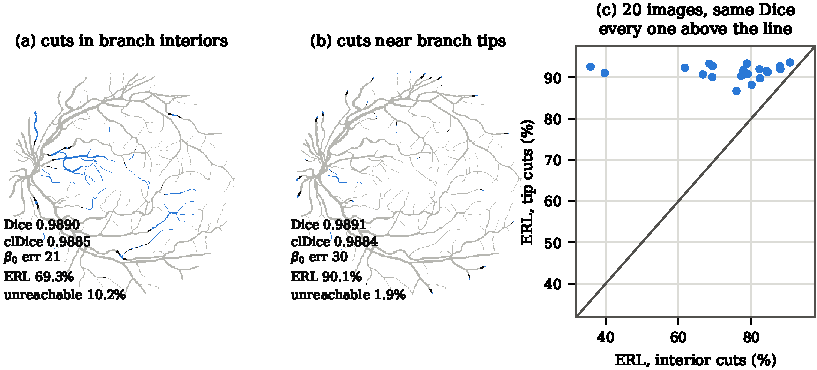
\includegraphics[width=\linewidth]{figures/fig1_case_set.pdf}
  \caption{The same mask, cut \csCuts{} times with the same discs at the same
  calibre; only the position along the branch differs. Black is the tissue
  removed, blue is what it cut off from the tree. (a) interiors, (b) tips ---
  both read Dice \csDice. (c) every one of \csImages{} images sits above the
  diagonal.}
  \label{fig:cases}
\end{figure}

\begin{table}[t]
  \centering
  \caption{A constructed case set on \csImages{} DRIVE test images,
  \csCuts{} cuts per arm. All four degraded arms delete the same area and
  post the same Dice. ``Unreachable'' is the quality anchor and is not
  derived from ERL. ERL convention: split\,/\,pixels\,/\,full.}
  \label{tab:cases}
  % tab1_case_set.tex -- GENERATED by exp/paper_figures.py. Do not edit here;
% edit the script, or the measurement it reads. Source: exp/results/blind_spot.csv, 20 DRIVE test images, 30 cuts per arm, ERL convention split/pixels/full, nothing selected on any split.
\begin{tabular}{lccccc}
\toprule
Arm & Dice & clDice & $\beta_0$ err & ERL & Unreach. \\
\midrule
ground truth & 1.0000 & 1.0000 & 0.0 & 98.1\% & 0.5\% \\
erosion, off centreline & 0.9889 & 1.0000 & 0.0 & 98.1\% & 0.5\% \\
erosion, anywhere & 0.9889 & 0.9963 & 0.0 & 59.9\% & 0.5\% \\
cuts near tips & 0.9889 & 0.9877 & 30.2 & 91.4\% & 1.4\% \\
cuts in interiors & 0.9889 & 0.9878 & 19.8 & 74.0\% & 11.1\% \\
\bottomrule
\end{tabular}

\end{table}

% The single most quotable sentence in the paper is the Betti-0 reversal.
% Do not bury it: \csBettiMid{} < \csBettiTip{}, lower is better, so Betti-0
% prefers the arm that orphans \csUnreachMid\% of the tree over the one that
% orphans \csUnreachTip\%.  The mechanism is measured, not argued: only
% \csSplitsMid{} of \csCuts{} interior cuts add a component, because
% \csLoopsMid{} of them fall on loops created where arteries and veins cross
% in projection.

\TODO{state the reversal, then give the loop mechanism}
% Budget: ~130 words. One paragraph. This is the quotable one.
\FILL{8}
